\subsection{Szövegformázás}

%53
\begin{frame}
  \begin{description}[m]
    \item[\texttt{text-align}] \hfill \\ Vízszintes igazítás: \texttt{left} (balra), \texttt{center} (középre), \texttt{right} (jobbra), \texttt{justify} (sorkizárt)
  \end{description}
  \begin{columns}[c]
    \column{0.6\textwidth}
      \begin{exampleblock}{\textattachfile{vizszintes.html}{vizszintes.html}}
        \tiny
        \lstinputlisting[style=HTML,linerange={7-10},numbers=left,firstnumber=7]{vizszintes.html}
        \lstinputlisting[style=HTML,linerange={15-16},numbers=left,firstnumber=15]{vizszintes.html}
      \end{exampleblock}
    \column{0.35\textwidth}
      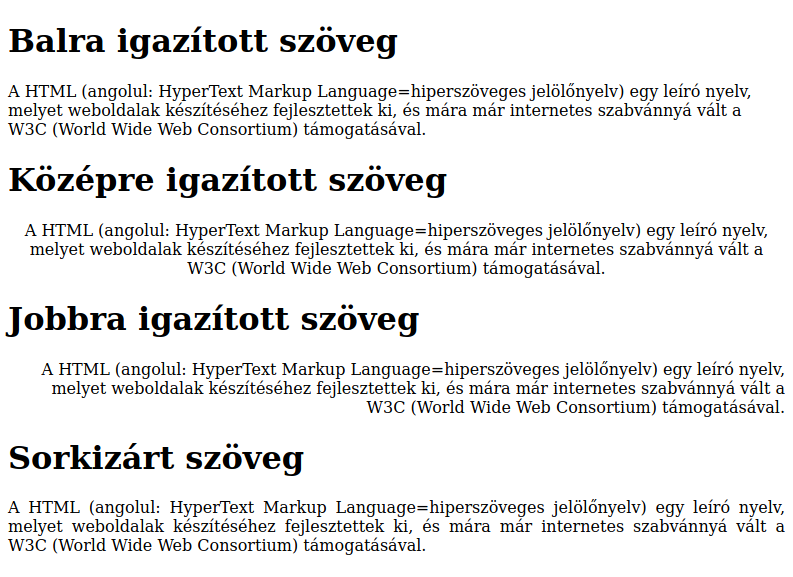
\includegraphics[width=\textwidth]{vizszintes.png}
  \end{columns}
\end{frame}

%54
\begin{frame}
  \texttt{vertical-align}: tetszőleges elem függőleges igazítása
  \begin{description}[m]
    \item[\texttt{baseline}] \hfill \\ szülő szövegének alapvonalához
    \item[\emph{távolság}] \hfill \\ tetszőleges mértékű süllyesztéshez/emeléshez, negatív érték is elfogadott
    \item[\texttt{\%}] \hfill \\ sormagasság \%-ában megadott emelés/süllyesztés, negatív érték is elfogadott
    \item[\texttt{sub}] \hfill \\ szülő alsó indexéhez
    \item[\texttt{super}] \hfill \\ szülő felső indexéhez
  \end{description}
\end{frame}

%55
\begin{frame}
  \begin{description}[m]
    \item[\texttt{top}] \hfill \\ sor legmagasabb eleméhez
    \item[\texttt{text-top}] \hfill \\ szülő elem szövegének tetejéhez
    \item[\texttt{middle}] \hfill \\ szülő közepéhez
    \item[\texttt{bottom}] \hfill \\  sor legalsó eleméhez
    \item[\texttt{text-bottom}] \hfill \\ szülő szövegének aljához
  \end{description}
\end{frame}

%56
\begin{frame}
  \begin{columns}[c]
    \column{0.55\textwidth}
      \begin{exampleblock}{\textattachfile{fuggoleges.html}{fuggoleges.html}}
        \tiny
        \lstinputlisting[style=HTML,linerange={7-9},numbers=left,firstnumber=7]{fuggoleges.html}
        \lstinputlisting[style=HTML,linerange={13-15},numbers=left,firstnumber=13]{fuggoleges.html}
      \end{exampleblock}
    \column{0.4\textwidth}
      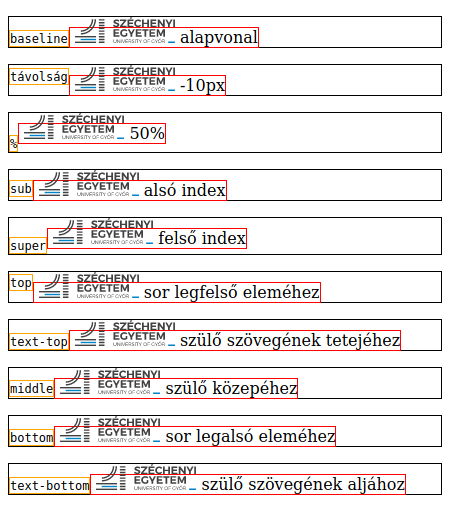
\includegraphics[width=\textwidth]{fuggoleges.png}
  \end{columns}
\end{frame}

%57
\begin{frame}
  \begin{description}[m]
    \item[\texttt{text-indent}] \hfill \\ Első sor behúzása: \emph{távolság} (a bekezdés bal szélétől számított behúzás), \texttt{\%} (szülő elem szélességének százalékában adott behúzás)
  \end{description}
  \begin{columns}[c]
    \column{0.6\textwidth}
      \begin{exampleblock}{\textattachfile{behuzas.html}{behuzas.html}}
        \tiny
        \lstinputlisting[style=HTML,linerange={7-10},numbers=left,firstnumber=7]{behuzas.html}
        \lstinputlisting[style=HTML,linerange={14-16},numbers=left,firstnumber=14]{behuzas.html}
      \end{exampleblock}
    \column{0.35\textwidth}
      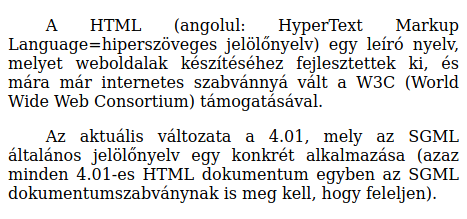
\includegraphics[width=\textwidth]{behuzas.png}
  \end{columns}
\end{frame}

%58
\begin{frame}
  \texttt{white-space}: fehér karakterek értelmezése
  \begin{description}[m]
    \item[\texttt{normal}] \hfill \\ szomszédos fehér karaktereket összevonja, alapértelmezés
    \item[\texttt{nowrap}] \hfill \\ nem tördeli a hosszú sorokat, de a szomszédos fehér karaktereket összevonja
    \item[\texttt{pre}] \hfill \\ utánozza a \texttt{<pre>} HTML elem működését, minden fehér karaktert megőriz
    \item[\texttt{pre-line}] \hfill \\ szomszédos fehér karaktereket összevonja, de tördeli a sorokat, ha szükséges
    \item[\texttt{pre-wrap}] \hfill \\ minden fehér karaktert megőriz, és tördel, ha szükséges
  \end{description}
\end{frame}

%59
\begin{frame}
  Nem választ magától \texttt{monospace} karakterkészletet!
  \begin{columns}[c]
    \column{0.6\textwidth}
      \begin{exampleblock}{\textattachfile{fahrcels2.html}{fahrcels2.html}}
        \footnotesize
        \lstinputlisting[style=HTML,linerange={7-10},numbers=left,firstnumber=7]{fahrcels2.html}
        \lstinputlisting[style=HTML,linerange={14-16},numbers=left,firstnumber=14]{fahrcels2.html}
      \end{exampleblock}
    \column{0.35\textwidth}
      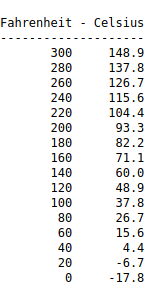
\includegraphics[width=0.7\textwidth]{fahrcels2.png}
  \end{columns}
\end{frame}

%60
\begin{frame}
  \texttt{letter-spacing}: betűk közötti távolság
  \begin{description}[m]
    \item[\texttt{normal}] \hfill \\ szokásos távolság, alapértelmezés
    \item[\emph{távolság}] \hfill \\ betűk közötti távolság, negatív érték is elfogadott
  \end{description}
  \vfill
  \texttt{word-spacing}: szavak közötti távolság
  \begin{description}[m]
    \item[\texttt{normal}] \hfill \\ szokásos távolság (betűmagasság negyede), alapértelmezés
    \item[\emph{távolság}] \hfill \\ szavak közötti távolság, negatív érték is elfogadott
  \end{description}
\end{frame}

%61
\begin{frame}
  \begin{exampleblock}{\textattachfile{tavolsag.html}{tavolsag.html}}
    \footnotesize
    \lstinputlisting[style=HTML,linerange={7-11},numbers=left,firstnumber=7]{tavolsag.html}
    \lstinputlisting[style=HTML,linerange={15-16},numbers=left,firstnumber=15]{tavolsag.html}
  \end{exampleblock}
  \begin{center}
    
\includegraphics[width=0.8\textwidth]{tavolsag.png}
  \end{center}
\end{frame}
